\chapter{Descripción del Trabajo}
\label{cap:descripcionTrabajo}

En cuanto al modelo de creación de imágenes a partir de una descripción, lo primero que se debe tener en cuenta es que tiene que ser de código abierto y gratuito, al que cualquier usuario tenga acceso. Además, tiene que ser acorde a la tarjeta gráfica de nuestro ordenador, una NVIDIA GeForce GTX 1050, con una memoria de vídeo dedicada de 3072 MB. Esta memoria es la encargada del almacenamiento y procesamiento de datos relacionados con la generación de imágenes y renderización de gráficos en una pantalla. Permite que la GPU acceda rápidamente a los datos necesarios para mejorar el rendimiento en aplicaciones de diseño, juegos y edición de vídeo.\\

Algunos modelos gratuitos, como el Stable Diffusion XL, generan imágenes con una calidad excepcional, pero tienen la limitación de que requieren una tarjeta gráfica demasiado desarrollada. Hemos utilizado esta herramienta en remoto y hemos probado sus funcionalidades de diferentes maneras. Se puede utilizar mediante código en Python a través de Google Colab y mediante la propia página de Stable Diffusion, que ofrece una demo para utilizar esta avanzada versión. Por último, también se puede utilizar en Hugging Face, que incluye multitud de modelos para descargar y utilizar y presenta muy buenos resultados. A partir de esta página hemos obtenido diferentes modelos que mencionaremos más adelante.\\

El hecho de probar un modelo de inteligencia artificial en un servidor no es concordante con nuestros objetivos del proyecto, puesto que necesitamos entrenar un modelo e incluirlo en una aplicación, de manera que el usuario pueda interactuar y conseguir imágenes personalizadas en un tiempo aceptable.\\

El proceso que hemos llevado a cabo es, en primer lugar, probar modelos en múltiples servidores web para ver cuál puede ser el más acorde con nuestro trabajo. 
En segundo lugar, a partir del modelo de generación de imágenes elegido, se debe ejecutar en nuestro ordenador y ver cuál es el rendimiento real. Esto quiere decir que la imagen debe generarse de manera correcta y no deformada, y debe incluir todos los elementos solicitados en la descripción introducida. Además, debe realizar esta generación en un tiempo adecuado.\\

La manera por la que optamos para simular la generación de imágenes desde nuestro ordenador es la instalación de una interfaz, llamada NMKD Stable Diffusion GUI. Esta herramienta nos permite ejecutar localmente cualquier modelo de generación de imágenes a partir de texto, e incluso permite aceptar imágenes como input. Para la ejecución, debemos seleccionar un modelo (el que viene dado por defecto es la versión 1.5 de Stable Diffusion), introducir una descripción y ajustar el número de pasos, que determinarán la duración de la generación y la calidad de la imagen, en función del modelo escogido y las limitaciones que presenta la tarjeta gráfica, que como hemos explicado es fundamental para esta tarea. Uno de los puntos a favor de esta interfaz, y que resulta de gran interés para nuestro proyecto, es que permite la utilización de modelos personalizados. \\

Para la personalización del modelo de Stable Diffusion hemos probado distintas vías y se ha llegado a distintos resultados y conclusiones:\\

LORA training: \\

Experiencia de entrenamiento:\\

Una de las vías de entrenamiento escogidas para desarrollar nuestro modelo ha sido LoRA (Low-Rank Adaptation of Large Language Models). Esta técnica favorece un equilibrio entre el tamaño del archivo y la eficiencia del propio entrenamiento.\\

La manera de funcionamiento es sencilla, puesto que se deberá cargar un conjunto de imágenes en Google Drive, y esto es lo único que tiene que hacer el usuario como requisito fundamental antes de comenzar el entrenamiento. No obstante, es de vital importancia saber cuáles son los parámetros que se deben ajustar para poder desarrollar el modelo de manera correcta.\
\
Se debe indicar el nombre del proyecto. Es muy importante, porque  aquí es donde obtendremos el resultado final, y es donde se debe incluir el dataset que mencionamos en el párrafo anterior. A continuación, el modelo a entrenar, como se ha explicado, hemos elegido el Stable Diffusion 1.5, por lo que es el que sirve de base para todos los entrenamientos escogidos. No obstante, esta técnica de entrenamiento tiene la peculiar característica de que se puede utilizar de base cualquier checkpoint desarrollado previamente, por lo que en caso de realizar un entrenamiento sobre personas, existe la posibilidad de elegir un modelo de base especializado en retratos. Esto garantiza que, seleccionando unas fotografías adecuadas y ajustando de manera correcta cada parámetro, los resultados sean bastante buenos.\\

Resultados:\\

Personas:\\
En cuanto al entrenamiento mediante Lora con personas, elegimos una que no fuese reconocida previamente por nuestro modelo de Stable Diffusion. Optamos por una actriz coreana llamada Hoyeon Jung. El siguiente paso fue crear nuestro propio conjunto de datos, formado por 10 imágenes y que se pueda apreciar la persona desde todos los ángulos posibles, con el objetivo de que el aprendizaje sea de mayor calidad. El tamaño debe ser igual o superior a 512 píxeles por cada dimensión, siendo la relación 1 a 1.
\begin{figure}[h]
	\centering
	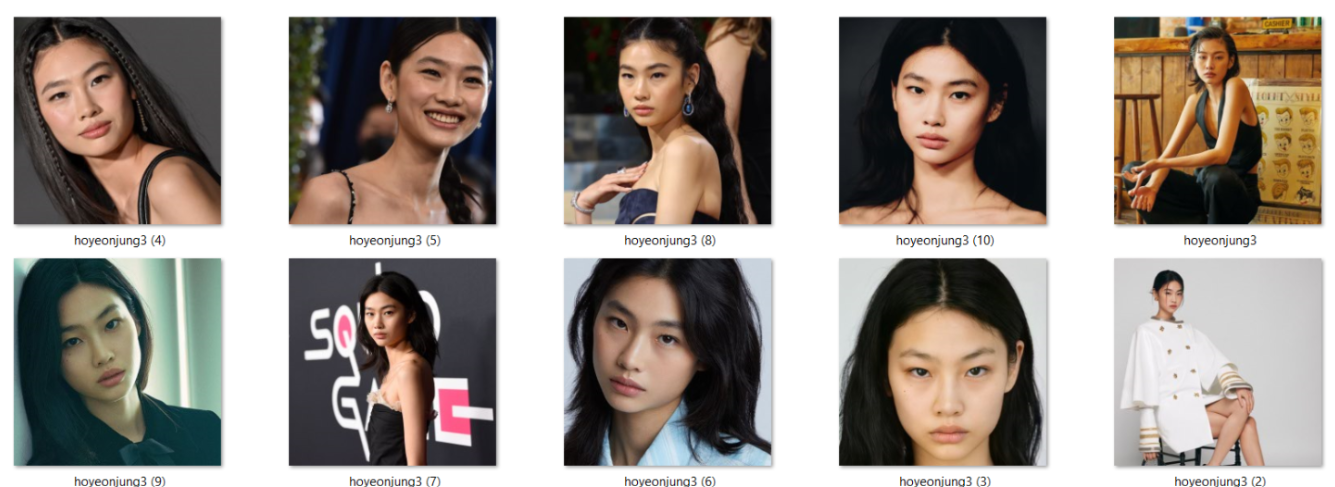
\includegraphics[width = 0.7
	\textwidth]{Imagenes/Vectorial/datasethoyeon.png}
	\caption{Dataset seleccionado para el entrenamiento de personas con Lora}
	\label{fig:sampleImage}
\end{figure}

Animales:\\
Para realizar una prueba del modelo de entrenamiento con Lora, lo primero fue elegir el animal y crear nuestro propio conjunto de datos, de manera que había que escoger 10 imágenes que tuviesen un tamaño igual o superior a 512 x 512 píxeles, y que la relación entre el ancho y el alto fuese 1 a 1. Además, al elegir el animal, se hizo la comprobación de que Stable Diffusion no lo incorporara ya en el modelo.\\ 
\begin{figure}[h]
	\centering
	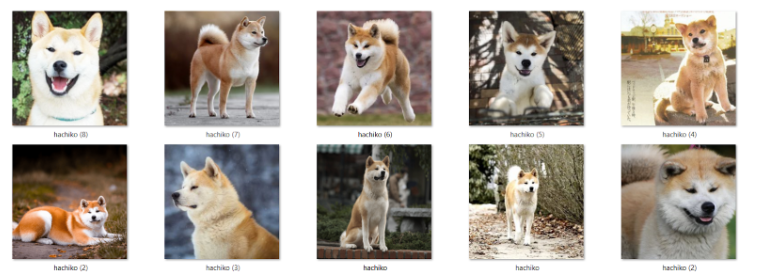
\includegraphics[width = 0.7
	\textwidth]{Imagenes/Vectorial/dataset_hachiko.png}
	\caption{Dataset seleccionado para el entrenamiento con animales}
	\label{fig:sampleImage}
\end{figure}

Como se puede apreciar en la figura anterior, se hizo hincapié en la diversidad de las imágenes, para aportar un mayor valor al entrenamiento, de modo que se tuviese una visión completa del elemento a entrenar.\\ 
Una vez entrenado el modelo, obtuvimos un total de 10 archivos en formato safetensor. Esto es debido a que, como hemos explicado con anterioridad, Lora tiene la ventaja de devolver múltiples resultados con un número de pasos distinto, con el objetivo de tener la posibilidad de probar cuáles son los steps ideales, y con cuáles habría falta o exceso de entrenamiento. En este caso, el safetensor adecuado fue el primero, puesto que a partir del segundo se podía apreciar la deformidad típica del sobreentrenamiento.\\
\begin{figure}[h]
	\centering
	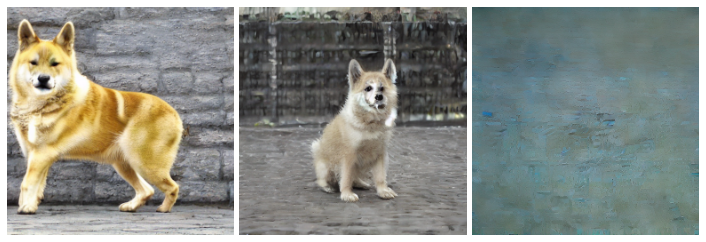
\includegraphics[width = 0.6
	\textwidth]{Imagenes/Vectorial/comparacion_hachiko.png}
	\caption{Mismo prompt con 1000, 2000 y 10.000 pasos de entrenamiento}
	\label{fig:sampleImage}
\end{figure}

En el momento en el que se descartan los demás archivos Safetensor, la siguiente labor es probar cuál es el número de pasos ideal para la generación de imágenes, y descubrir si con diferentes prompts, el modelo entrenado podría obtener buenos resultados.\\

\begin{figure}[h]
	\centering
	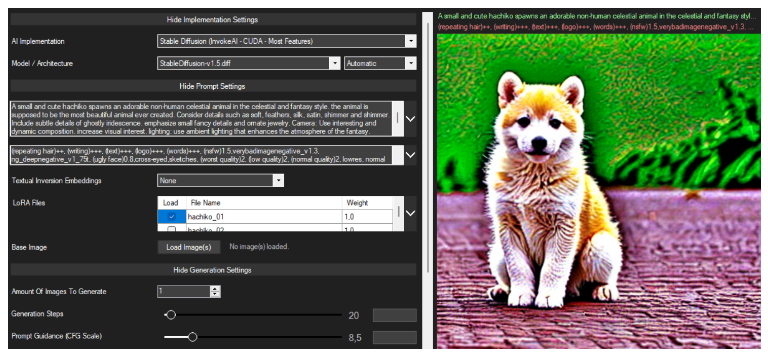
\includegraphics[width = 0.6
	\textwidth]{Imagenes/Vectorial/hachiko_detallada.png}
	\caption{Imagen generada con el modelo Stable Diffusion 1.5, Lora Hachiko}
	\label{fig:sampleImage}
\end{figure}

Aspectos a tener en cuenta:\\


Dreambooth:\\
Para el entrenamiento, teníamos el objetivo de lograr que el modelo pudiera generar imágenes personalizadas propias con cierta calidad y en un tiempo aceptable, y eso es lo que consideramos éxito.\\
Hemos logrado entrenar un modelo de generación de imágenes incluyendo fotografías propias, y eso es algo que puede ser realmente útil para nuestros propósitos. Esto es porque podemos lograr que cualquier persona pueda incorporar las imágenes que considere oportunas para servir de apoyo al paciente. A continuación, procederemos a explicar cómo ha sido el entrenamiento y los pasos que se han de seguir para lograr un resultado exitoso.\\

Como recordatorio, de los modelos de Stable Diffusion empleados, la versión que resultó mejor a nivel de creación de imágenes en un tiempo aceptable fue la 1.5. Una vez seleccionado el modelo que debíamos potenciar, lo siguiente fue decidir el método de entrenamiento. Optamos por el modelo de Dreambooth, el cuál nos permite añadir capas de entrenamiento a la inteligencia artificial para que reconozca objetos concretos. Esto es muy importante, porque es la manera de adaptar la inteligencia artificial a la utilización que queremos otorgarle.\\

Dreambooth es un modelo de generación de aprendizaje profundo, y que fue desarrollado en 2022 por un grupo de investigadores de Google Research y la Universidad de Boston. La misión de esta tecnología es la de poder entrenar a modelos de inteligencia artificial para personalizarlo según tus necesidades.\\


Los pasos para el entrenamiento son claros y sencillos. En primer lugar, debemos tener claro el elemento o token al que queremos dar una identidad. Por ejemplo, si seleccionamos una persona, debemos elegir unas imágenes en las que aparezca, de tal manera que, tras el entrenamiento, la IA pueda identificarla. Lo ideal es que se elija un número considerable de fotografías, a partir de 10. Estas deberán tener un tamaño exacto de 500 x 500 píxeles, y deberán llamarse exactamente de la misma manera, con el identificador del token al que hagamos referencia.\\

Una vez tengamos seleccionadas todas las imágenes, debemos utilizar el código abierto en la plataforma Google Colab para realizar el entrenamiento. Tras la finalización, se creará un archivo de alrededor de 2 gigabytes, que contendrá el modelo de Stable Diffusion 1.5, con una capa de entrenamiento más, puesto que incorporará el elemento deseado. Con esto ya tendríamos un elemento de inteligencia artificial personalizado.\\
\begin{figure}[h]
	\centering
	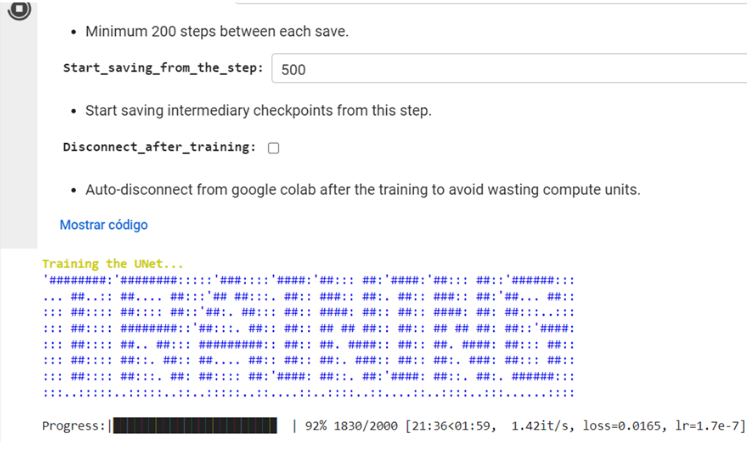
\includegraphics[width = 0.4
	\textwidth]{Imagenes/Vectorial/dreambooth.png}
	\caption{Procedimiento del entrenamiento mediante Dreambooth}
	\label{fig:sampleImage}
\end{figure}


Este archivo, en formato ckpt, se podrá utilizar en la aplicación para generar imágenes, y contendrá el elemento entrenado. Si posteriormente se pretende incluir elementos al modelo ya entrenado, también se puede realizar realizando un nuevo entrenamiento utilizando de base el archivo en ckpt anterior. Cuando se realice este segundo entrenamiento, se podrán generar imágenes acerca de ambos elementos, lo cuál es muy útil para nuestros objetivos, ya que en un mismo modelo enfocado a un paciente, debe haber múltiples elementos.\\

Un aspecto muy importante a tener en cuenta, es que tras haber realizado múltiples pruebas, los resultados óptimos los hemos obtenido seleccionando un conjunto de datos formado por 10 imágenes, y con 2400 pasos de entrenamiento.\\

En cuanto a resultados:\\
Personas: Resultado correcto. Se ha conseguido mostrar de forma clara y nítida a la persona con la que se ha entrenado el modelo, con un prompt y número de pasos adecuado.\\
\begin{figure}[h]
	\centering
	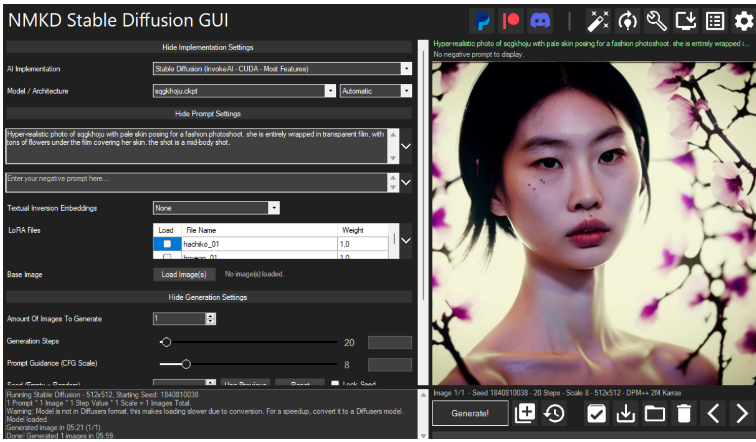
\includegraphics[width = 0.5
	\textwidth]{Imagenes/Vectorial/hoyeon1.png}
	\caption{Resultados de entrenamiento de una persona con Dreambooth}
	\label{fig:sampleImage}
\end{figure}

\begin{figure}[h]
	\centering
	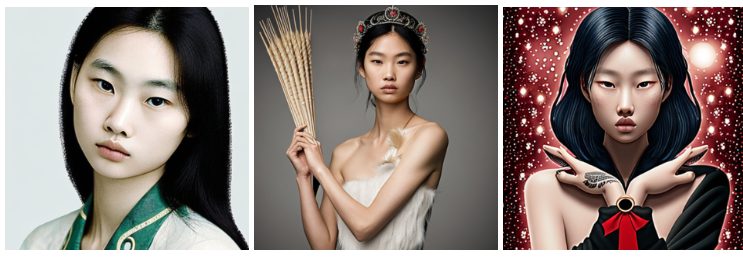
\includegraphics[width = 0.6
	\textwidth]{Imagenes/Vectorial/hoyeon_results.png}
	\caption{Resultados de entrenamiento de una persona con diferentes estilos}
	\label{fig:sampleImage}
\end{figure}
Lugares concretos: Resultado correcto. Calidad de la imagen muy buena. Permite establecer múltiples estilos y el edificio se puede visualizar a la perfección. Es algo que aporta muchísimo valor a nuestro modelo, y que cumple con los requisitos establecidos previamente.\\

Hemos entrenado nuestro modelo con un edificio característico, que por supuesto no estuviera incluido previamente. Se trata de la basílica de Colmenar Viejo, Madrid. El dataset seleccionado para que se pudiera observar el edificio en su totalidad, desde diferentes perspectivas, es el siguiente:\\\\\\\\\\

\begin{figure}[!htb]
	\centering
	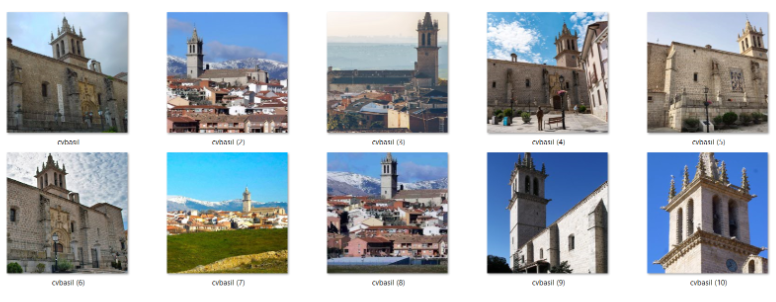
\includegraphics[width = 0.7
	\textwidth]{Imagenes/Vectorial/dataset_colmenar.png}
	\caption{Dataset seleccionado para el entrenamiento con lugares}
	\label{fig:sampleImage}
\end{figure}

Con diferentes estilos:\\

\begin{figure}[!htb]
	\centering
	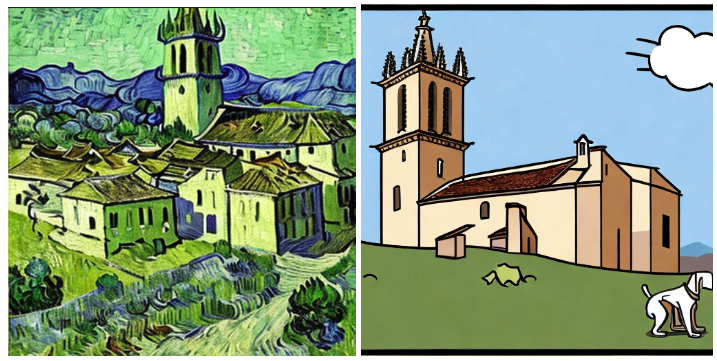
\includegraphics[width = 0.6
	\textwidth]{Imagenes/Vectorial/colmenar_styles.png}
	\caption{Resultados de imagenes del lugar entrenado al estilo Van Gogh y viñeta}
	\label{fig:sampleImage}
\end{figure}


Añadiendo otros elementos:\\


\begin{figure}[!htb]
	\centering
	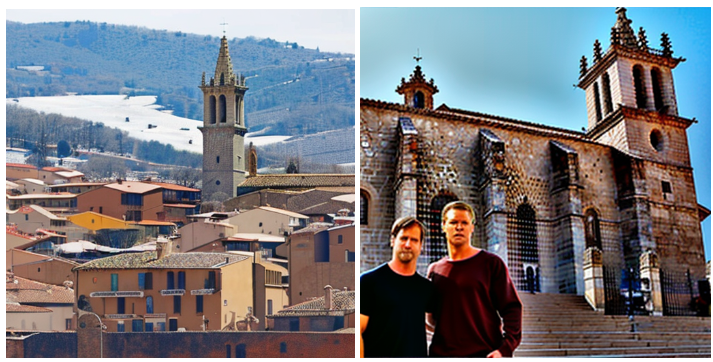
\includegraphics[width = 0.6
	\textwidth]{Imagenes/Vectorial/colmenar_elements.png}
	\caption{Resultados de imágenes del lugar en invierno y con una persona}
	\label{fig:sampleImage}
\end{figure}


Peligros con el sobreentrenamiento: Se produce cuando el modelo no se puede generalizar y se ajusta demasiado al conjunto de datos entrenados. Se debe principalmente a que el tamaño de los datos es demasiado pequeño y no contiene suficientes muestras de datos para poder representar con precisión la totalidad de datos de entrada posibles. Otra razón es que el modelo se entrena durante demasiado tiempo en un solo conjunto de datos de muestra. En nuestro modelo, encontramos sobreentrenamiento cuando elegimos un número de steps muy elevado para un número de fotografías que no es lo suficientemente alto. Una manera de detectar que nuestro modelo está sobreentrenado es cuando no genera bien la cara de la persona, y se aprecian fallos en determinadas facciones, como en los ojos y la boca, en los cuales se aprecia deformidad.\\

Falta de pasos en el entrenamiento: En este caso, se produce cuando el modelo de datos no tiene la capacidad de capturar de forma precisa la relación entre las variables de entrada y de salida, de manera que existe un elevado índice de errores en el conjunto de datos de entrenamiento y en los datos no vistos. Se debe a que el modelo es demasiado simple, porque el tamaño de los datos es demasiado pequeño, o bien porque se necesita más tiempo de entrenamiento. En este caso, cuando generamos las imágenes, se evidencia que el modelo aún no ha aprendido lo suficiente acerca del elemento o token del que se ha realizado el entrenamiento, pues el resultado de la generación refleja una persona que no muestra ningún parecido con la realidad.\\

En cuanto a mezcla de personas: Para ampliar los horizontes de nuestro entrenamiento, hemos entrenado a una persona, asociando un token a ella para su identificación, sobre un modelo que previamente ya había sido entrenado con una persona y su token asociado, para comprobar si efectivamente se podía generar en una sola imagen una representación de las dos personas entrenadas, una junto a la otra. Es aquí donde se ha detectado una peculiaridad, ya que, a pesar de que un modelo genere buenos resultados de cada una de las dos personas, en el mismo momento que se solicita en un determinado prompt o descripción que se vean reflejados una o varias personas entrenadas en la misma fotografía, ningún modelo de los que se haya probado, ha generado buenos resultados de esta manera. Lo que finalmente se aprecia en la imagen generada, es que aparecen dos personas pero sus rostros son una mezcla de las características faciales y fisiológicas de ambas, produciéndose una deformidad en muchos de los casos y que los rostros aparezcan prácticamente duplicados.
\begin{figure}[h]
	\centering
	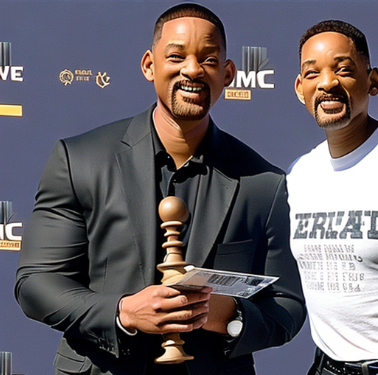
\includegraphics[width = 0.4
	\textwidth]{Imagenes/Vectorial/duplicidad_will.png}
		\caption{Duplicidad de elementos}
	\label{fig:sampleImage}
\end{figure}

Avances respecto al modelo.\\

Aplicación de Stable Diffusion genera imágenes aceptables en un tiempo normal (1-2 minutos como máximo). Existe la posibilidad de utilizar imágenes para poder incorporar al modelo de Stable Diffusion como Token. La aplicación contiene un apartado de training, pero tras probar incorporar escasas imágenes al modelo, el proceso es demasiado largo (varios días) y el resultado es una incógnita. \\

El modelo de .csv parece estar obsoleto, y al intentar el entrenamiento con las imágenes de personas sale un error en el paso 6, lo cual limita y habrá que identificar y trabajar con otro modelo de entrenamiento. LoRA puede ser una opción para ello.
También hemos probado más modelos de Hugging Face a ejecutar por consola mediante Anaconda, pero los resultados no son los adecuados. Generan imágenes de calidad no muy buena en un tiempo muy elevado, entre 10 y 20 minutos. Por tanto, también decidimos descartar esta vía. 
La más razonable hasta ahora es la GUI de Stable Diffusion, ya que es la única que genera imágenes en un tiempo adecuado, y que permite la posibilidad de incorporar imágenes propias al modelo\\




 Como muestra la figura \ref{fig:sampleImage},
